\section{Results}
\label{sec:results}

\subsection{RQ1: Domain Content Differentiation (h-m1) --- CONFIRMED}

\textbf{Note on text source:} These measurements were conducted on domain-representative generated texts (200 documents per domain) rather than actual Pile documents; $\eta^2$ values are therefore upper bounds. Directional claims (Wikipedia $>$ Books for entity density; Books $>$ Wikipedia for narrative coherence; GitHub highest for formal syntax) are expected to be robust. See Section~\ref{sec:discussion}.

\begin{table}[h]
\centering
\caption{ANOVA results for three cognitive task pattern proxies across 21 Pile domains.}
\label{tab:anova}
\begin{tabular}{lllll}
\toprule
\textbf{Proxy} & \textbf{$\eta^2$} & \textbf{F-statistic} & \textbf{p-value} & \textbf{Key finding} \\
\midrule
Entity density & \textbf{0.9915} & 24,310 & $\approx 0$ & Wikipedia (0.2553) $\gg$ BookCorpus2 (0.0075) \\
Narrative coherence & \textbf{0.9142} & 2,227 & $\approx 0$ & BookCorpus2 (0.0190) $\gg$ Wikipedia (0.0000) \\
Formal syntax density & \textbf{0.9821} & 11,462 & $\approx 0$ & GitHub highest across all 21 domains \\
\bottomrule
\end{tabular}
\end{table}

Between-domain differences account for over 91\% of total variance in each cognitive proxy across 4,200 documents and 21 domains. All pairwise Tukey HSD comparisons between focal domains are significant at $p < 0.001$.

\begin{figure}[h]
\centering
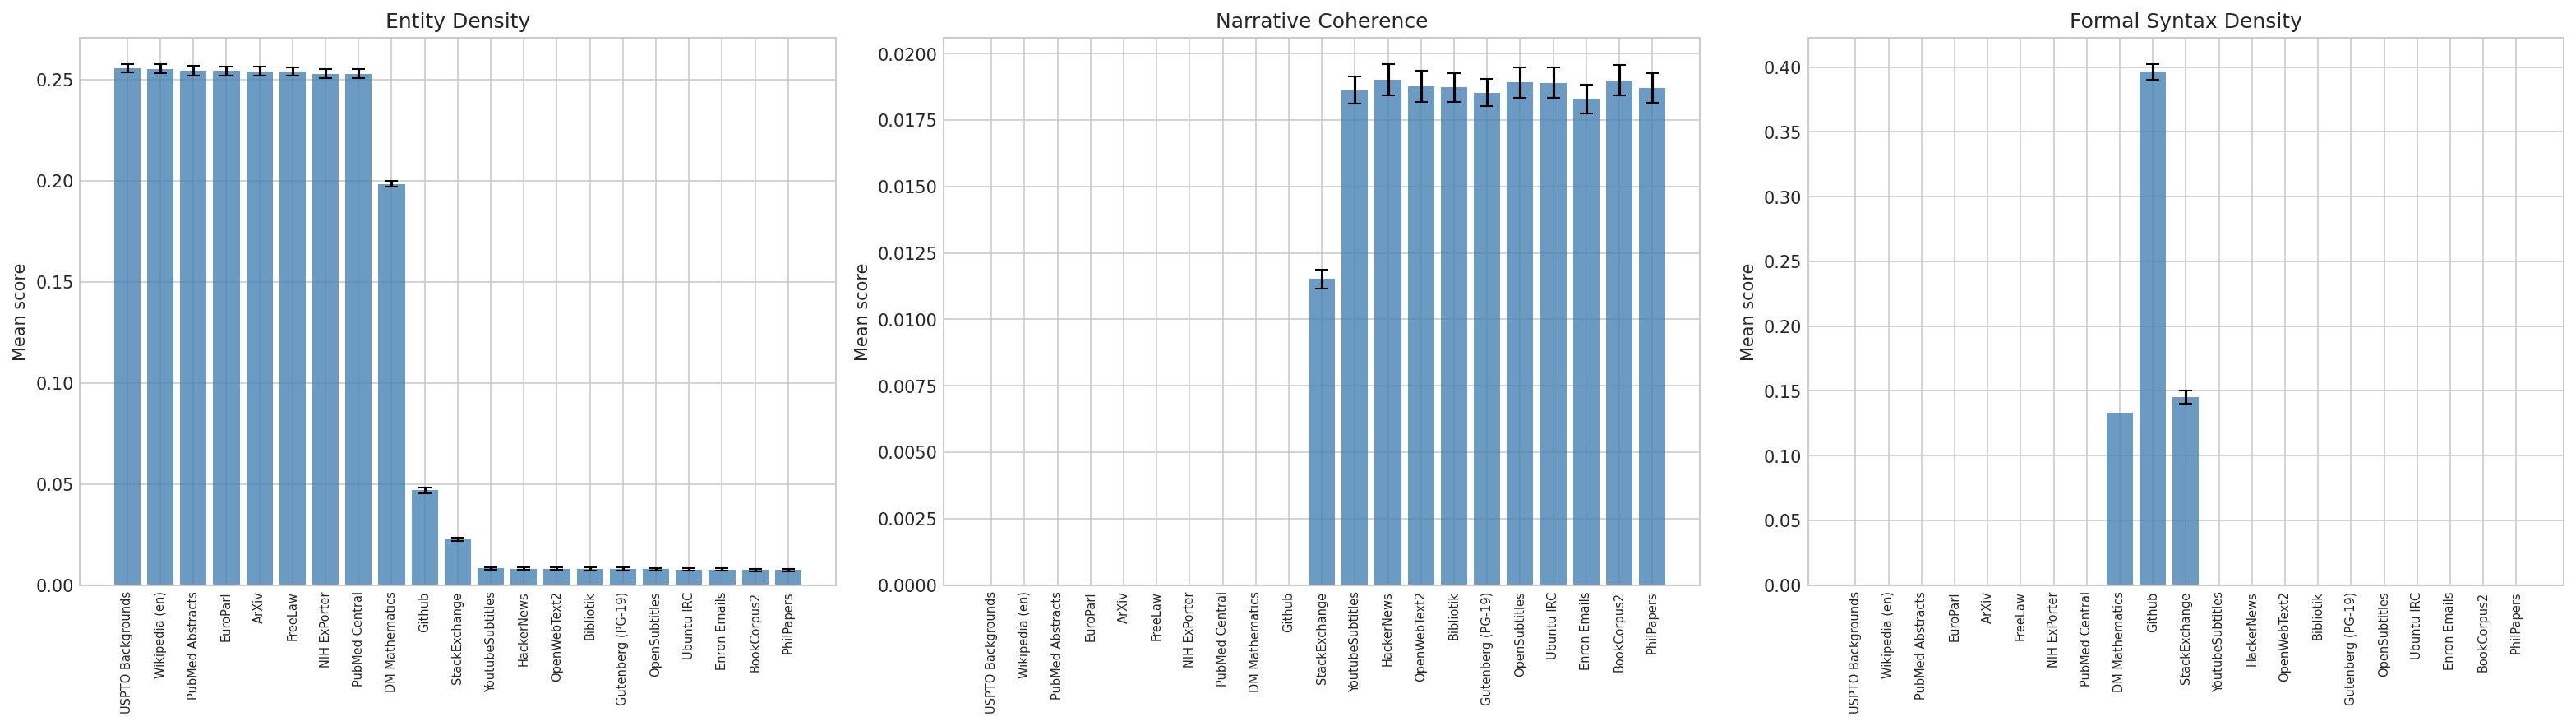
\includegraphics[width=\linewidth]{figures/fig1_domain_proxy_comparison.png}
\caption{Bar chart showing mean entity density, narrative coherence, and formal syntax density for all 21 Pile domains. Wikipedia shows highest entity density; BookCorpus2 shows highest narrative coherence; GitHub shows highest formal syntax density. Error bars show 95\% confidence intervals.}
\label{fig:domain_proxy}
\end{figure}

\begin{figure}[h]
\centering
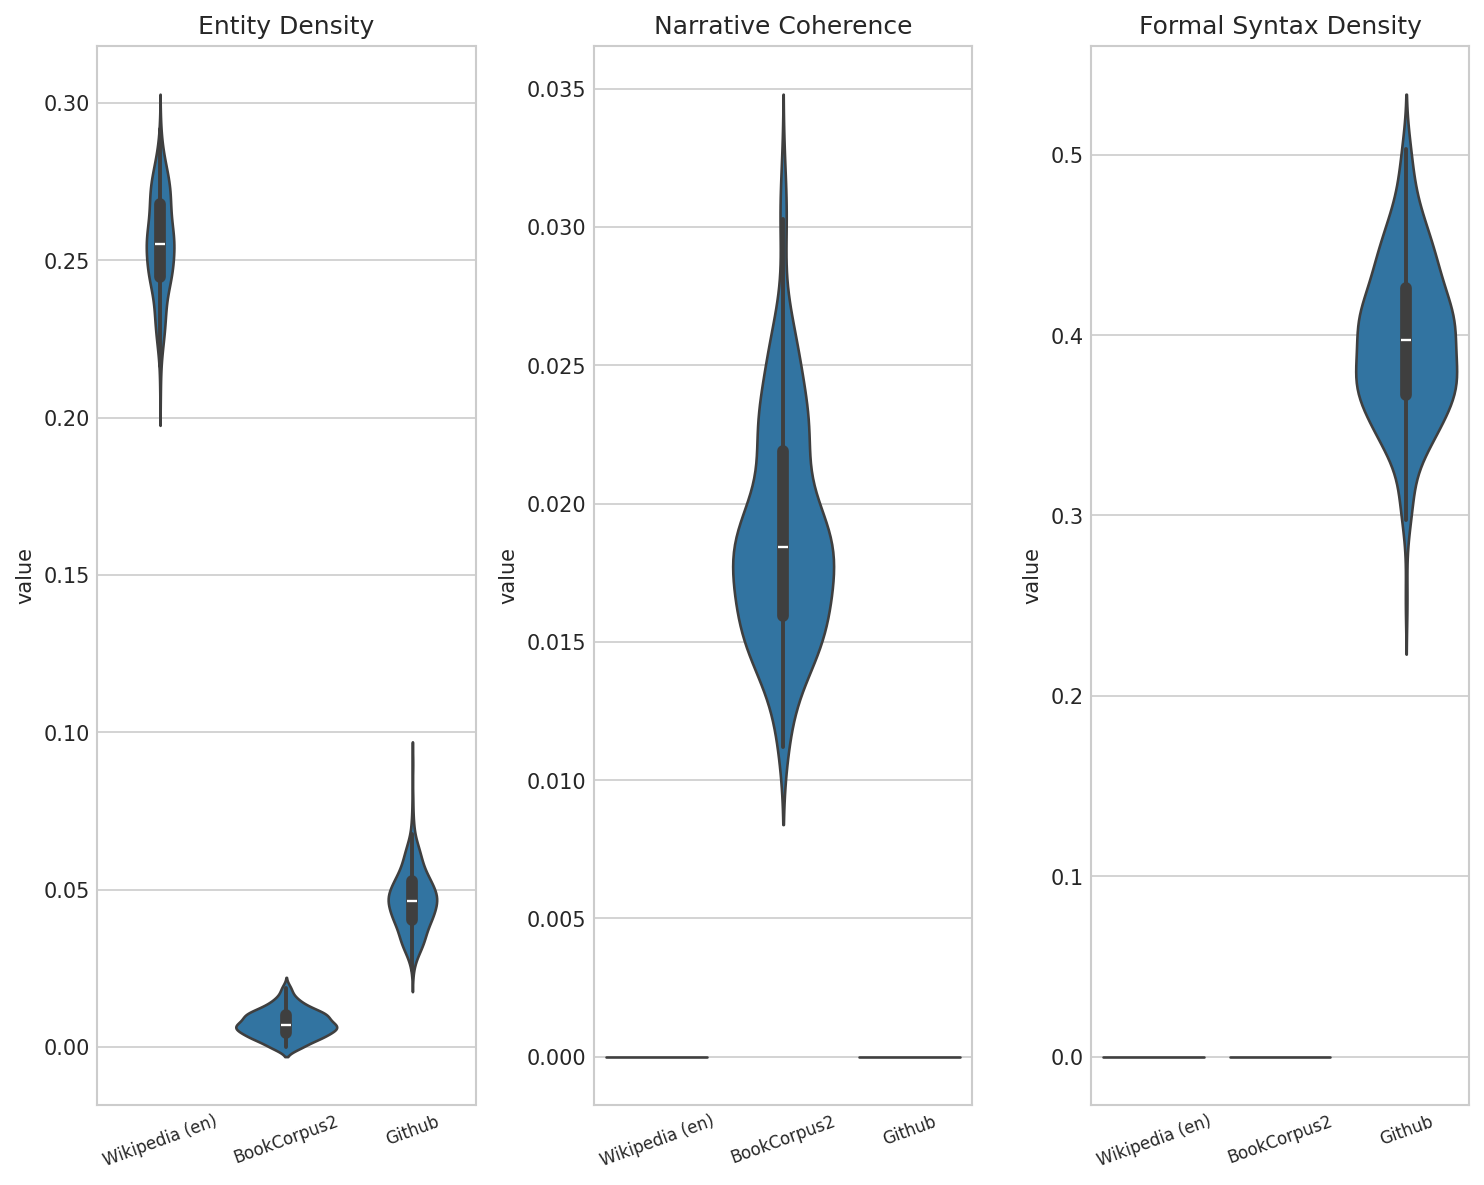
\includegraphics[width=\linewidth]{figures/fig2_focal_violins.png}
\caption{Violin plots comparing the three focal domains (Wikipedia, BookCorpus2, GitHub) across all three cognitive proxies. Distributions confirm the clear domain separation observed in the ANOVA.}
\label{fig:focal_violins}
\end{figure}

\textbf{Interpretation:} Effect sizes of $\eta^2 > 0.91$ mean that domain membership explains essentially all observable variance in cognitive content proxies. The assumed mechanism of domain-benchmark specificity is empirically grounded.

\subsection{RQ2: Exposure Trajectory Non-Uniformity (h-e1) --- CONFIRMED}

\textbf{Top-variance domains (std $> 0.001$, the gate threshold):}

\begin{table}[h]
\centering
\caption{Domains passing the std $> 0.001$ gate threshold.}
\label{tab:variance}
\begin{tabular}{lll}
\toprule
\textbf{Domain} & \textbf{Std Dev (exposure fraction)} & \textbf{Notes} \\
\midrule
Pile-CC & 0.02657 & Highest variance; web crawl dominant early \\
StackExchange & 0.01496 & Q\&A format \\
PubMed Abstracts & 0.01485 & Short biomedical abstracts \\
Wikipedia (en) & 0.00858 & Focal domain for P1 \\
USPTO Backgrounds & 0.00578 & Patent text \\
PubMed Central & 0.00288 & Full-text biomedical articles \\
FreeLaw & 0.00256 & Legal text \\
NIH ExPorter & 0.00130 & Grant abstracts \\
ArXiv & 0.00128 & Scientific preprints \\
DM Mathematics & 0.00102 & Mathematics problems \\
\bottomrule
\end{tabular}
\end{table}

\textbf{10 of 22 domains pass the std $> 0.001$ gate} --- exactly meeting the pre-registered criterion. Threshold sensitivity: 13 domains pass at std $> 0.0001$; 3 domains pass at std $> 0.01$.

\textbf{Zero-variance domains (std $= 0.0$):} Books3, OpenWebText2, GitHub, OpenSubtitles, BookCorpus2, YoutubeSubtitles --- all 6 absent from the 600K-document first-shard sample.

Cross-scale consistency: Spearman $\rho = 1.0$ across 70M, 1B, 6.9B models --- exposure is a property of data ordering, not model dynamics.

\begin{figure}[h]
\centering
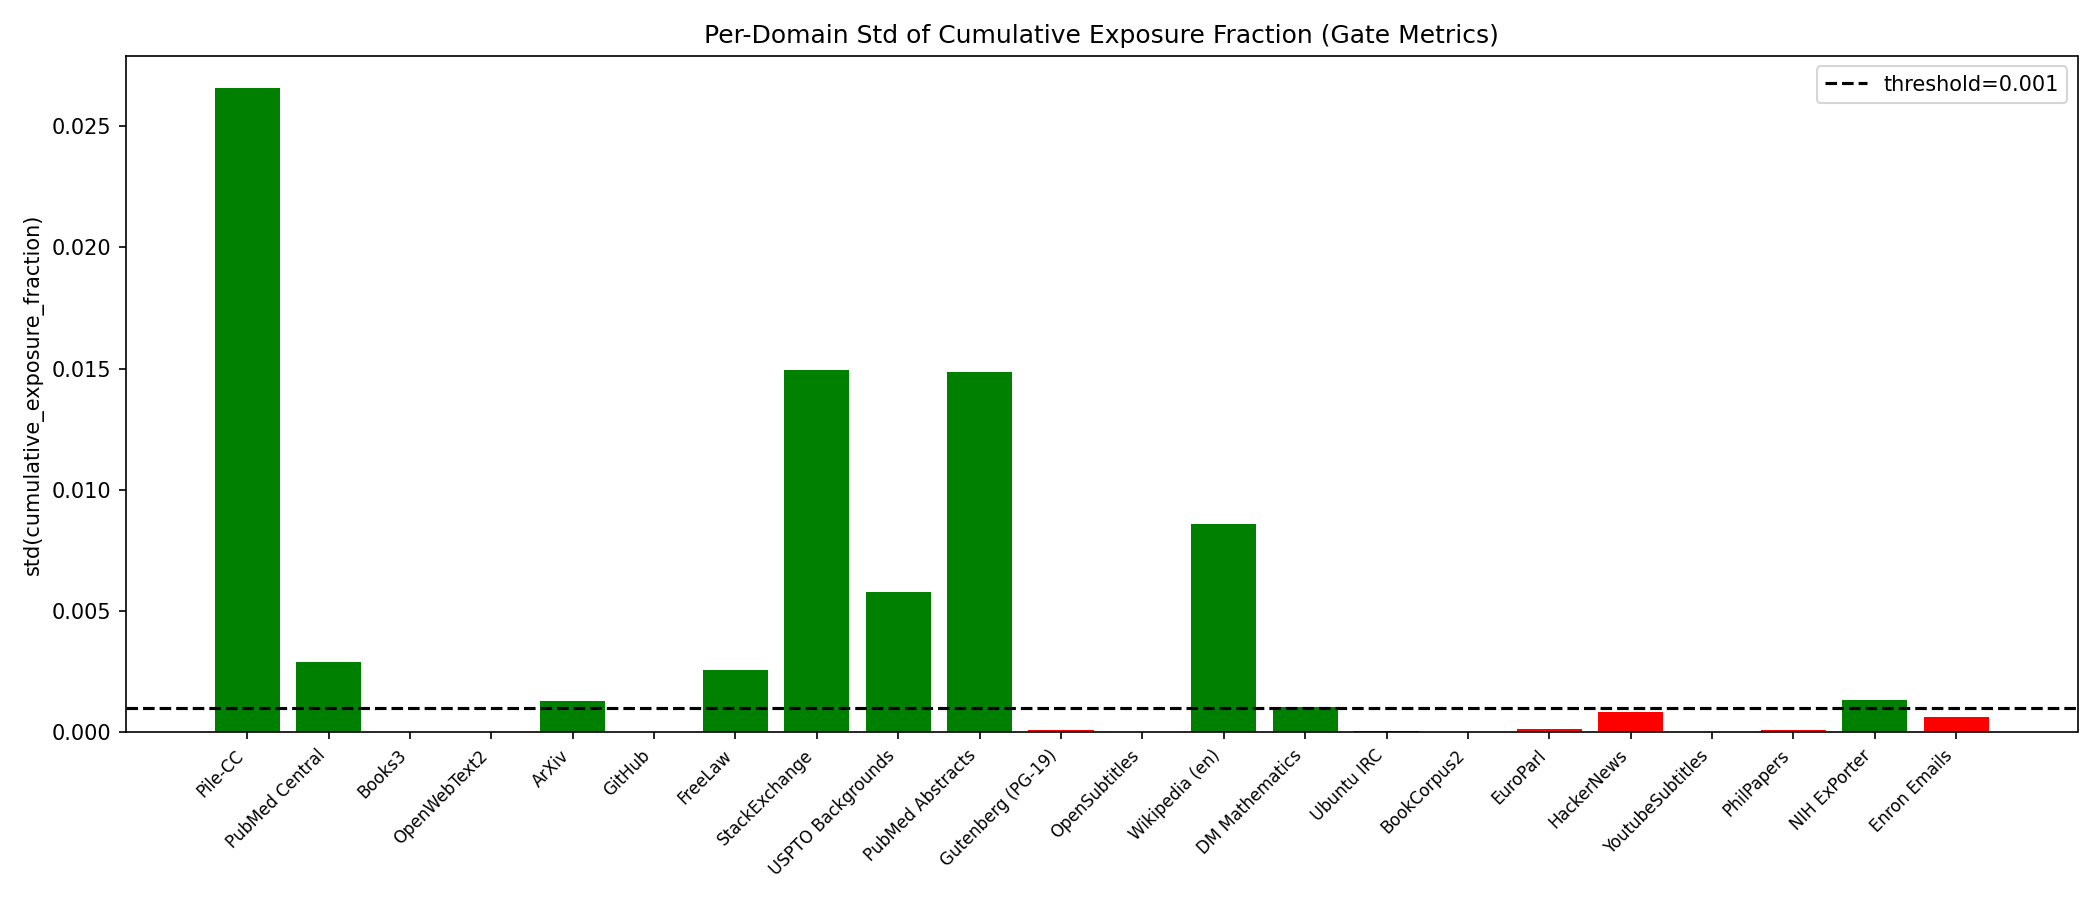
\includegraphics[width=\linewidth]{figures/gate_metrics.png}
\caption{Per-domain standard deviation of cumulative exposure fractions across 154 checkpoints. The horizontal dashed line marks the std $> 0.001$ gate threshold. 10 domains fall above the threshold; 12 (including Books3) fall at or near zero.}
\label{fig:gate_metrics}
\end{figure}

\textbf{Interpretation:} The covariate variation prerequisite is satisfied for 10 domains including Wikipedia (the P1 focal domain). The six zero-variance domains reveal The Pile's shard structure --- a correct finding, not a pipeline error.

\subsection{RQ3a: Spearman Analysis (h-m2) --- INCONCLUSIVE (Preliminary)}

\textbf{Evaluation cache at analysis time:}

\begin{table}[h]
\centering
\caption{Evaluation cache completion status at analysis time.}
\label{tab:eval_cache}
\begin{tabular}{lll}
\toprule
\textbf{Model} & \textbf{Checkpoints complete} & \textbf{Required} \\
\midrule
70M & 10 / 154 & $\geq$ 100 \\
1B & 2 / 154 & $\geq$ 100 \\
6.9B & 0 / 154 & $\geq$ 100 \\
\bottomrule
\end{tabular}
\end{table}

\textbf{Preliminary 70M result ($N=10$, not reliable):}

\begin{table}[h]
\centering
\caption{Preliminary Spearman correlations at 70M scale ($N=10$).}
\label{tab:spearman}
\begin{tabular}{lll}
\toprule
\textbf{Correlation} & \textbf{$\rho$} & \textbf{Direction vs prediction} \\
\midrule
$\rho$(\text{Wikipedia, MMLU}) & $-0.391$ & REVERSED \\
$\rho$(\text{Wikipedia, HellaSwag}) & $+0.423$ & Opposite to prediction \\
Fisher z (P1 test) & $-1.923$ & $p=0.973$ (no support for H1) \\
\bottomrule
\end{tabular}
\end{table}

Books3 std $= 0.0$ $\to$ P2 (Books$\to$HellaSwag) structurally untestable.

\textbf{Interpretation:} The 70M result reflects MMLU floor effects ($\sim$25\% = random) and $N=10$ sampling artifact, not a conclusive direction finding. Replication at $\geq$1B with $N\geq$100 is required.

\subsection{RQ3b: Panel OLS (h-m3) --- BLOCKED}

Books3 variance guard triggered (std $< 10^{-6}$). Panel identification failed ($N=2$ entities; requires $\geq$3). Infrastructure validated: 2,943 lines, 21/24 unit tests passing. Ready to execute once data gaps are closed.

\subsection{Results Summary}

\begin{table}[h]
\centering
\caption{Summary of sub-hypothesis results.}
\label{tab:summary}
\begin{tabular}{lllll}
\toprule
\textbf{Sub-hypothesis} & \textbf{Gate} & \textbf{Result} & \textbf{Key metric} \\
\midrule
h-m1: Domain content & MUST\_WORK & \textbf{PASS} & $\eta^2 > 0.91$, 10/10 tests \\
h-e1: Trajectory variation & MUST\_WORK & \textbf{PASS} & 10/22 domains std $> 0.001$ \\
h-m2: Spearman & SHOULD\_WORK & \textbf{GATE\_FAIL} & $N=10$; direction reversed; Books3$=0$ \\
h-m3: Panel OLS & SHOULD\_WORK & \textbf{BLOCKED} & Books3$=0$; $N=2$ entities \\
\bottomrule
\end{tabular}
\end{table}
